\documentclass[tikz,border=4pt]{standalone}
% Estilo común de los diagramas de bloques (se usa con \input en cada standalone)
\usepackage[defaultsans,scale=0.92]{lato}
\usepackage{libertinust1math}
\usepackage{xcolor,amsmath}
\usepackage{tikz}
\usetikzlibrary{positioning,arrows.meta,calc,shapes.geometric}
\usepackage{../../notacion}
\definecolor{ctrlazul}{HTML}{1E5AA8}\definecolor{ctrlnoche}{HTML}{14213D}
\definecolor{ctrlcoral}{HTML}{D1495B}\definecolor{ctrlverde}{HTML}{2A9D8F}
\definecolor{ctrlambar}{HTML}{E09F3E}\definecolor{ctrlgris}{HTML}{5C677D}
\definecolor{ctrlvioleta}{HTML}{6C4AB6}\definecolor{ctrlteal}{HTML}{0F7173}
\tikzset{
  >={Stealth[length=2.4mm]}, every node/.style={font=\small},
  bloque/.style={draw=ctrlnoche,fill=ctrlazul!7,thick,rounded corners=1.5pt,minimum height=9mm,minimum width=13mm,inner sep=4pt},
  suma/.style={draw=ctrlnoche,thick,circle,inner sep=0pt,minimum size=6mm},
  senal/.style={->,thick,draw=ctrlnoche},
  rot/.style={font=\footnotesize,text=ctrlgris},
}

\begin{document}
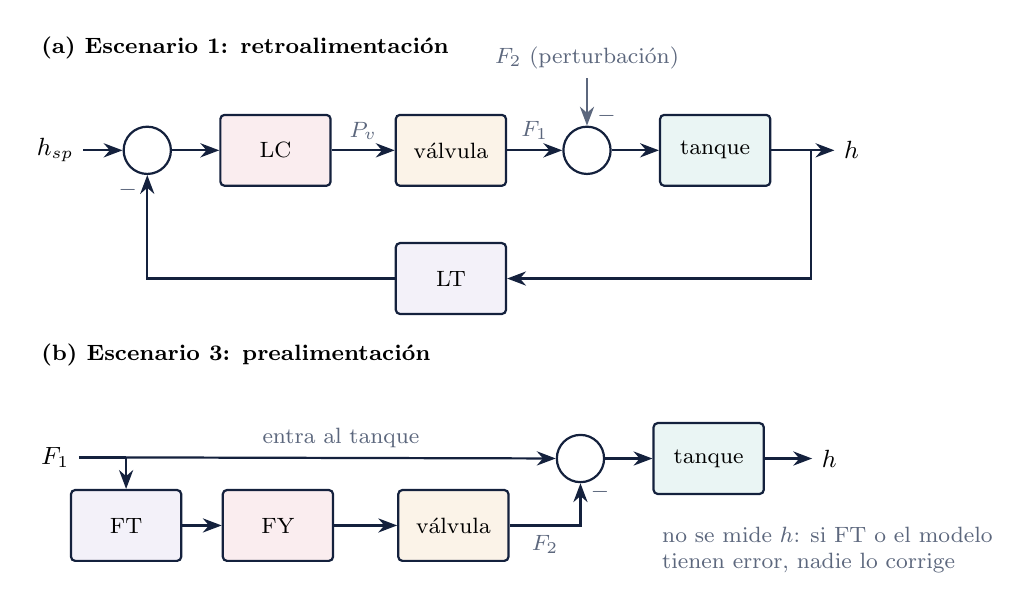
\begin{tikzpicture}[node distance=8mm, b/.style={bloque,minimum width=14mm,font=\footnotesize,align=center}]
  \node[font=\footnotesize\bfseries,anchor=west] at (-0.3,1.3) {(a) Escenario 1: retroalimentación};
  \node (r) at (0,0) {$h_{sp}$};
  \node[suma,right=5mm of r] (S) {};
  \node[b,right=6mm of S,fill=ctrlcoral!10] (c) {LC};
  \node[b,right=of c,fill=ctrlambar!12] (v) {válvula};
  \node[suma,right=7mm of v] (s1) {};
  \node[b,right=6mm of s1,fill=ctrlverde!10] (p) {tanque};
  \coordinate[right=5mm of p] (o); \node[right=3mm of o] (y) {$h$};
  \node[above=6mm of s1,rot] (d) {$F_2$ (perturbación)};
  \node[b,below=7mm of v,fill=ctrlvioleta!8] (lt) {LT};
  \draw[senal] (r)--(S); \draw[senal] (S)--(c);
  \draw[senal] (c)--node[above,rot]{$P_v$}(v);
  \draw[senal] (v)--node[above,rot]{$F_1$}(s1); \draw[senal] (s1)--(p);
  \draw[thick,draw=ctrlnoche] (p)--(o); \draw[senal] (o)--(y);
  \draw[senal,draw=ctrlgris] (d)--node[pos=0.8,right,rot]{$-$}(s1);
  \draw[senal] (o)|-(lt); \draw[senal] (lt)-|node[pos=0.93,left,rot]{$-$}(S);
  \begin{scope}[yshift=-3.9cm]
  \node[font=\footnotesize\bfseries,anchor=west] at (-0.3,1.3) {(b) Escenario 3: prealimentación};
  \node (F1) at (0,0) {$F_1$};
  \coordinate[right=6mm of F1] (k);
  \node[b,below=4mm of k,fill=ctrlvioleta!8,anchor=north] (ft) {FT};
  \node[b,right=5mm of ft,fill=ctrlcoral!10] (ff) {FY};
  \node[b,right=of ff,fill=ctrlambar!12] (v) {válvula};
  \node[suma] (s1) at ($(v.east)+(9mm,0.85)$) {};
  \node[b,right=6mm of s1,fill=ctrlverde!10] (p) {tanque};
  \node[right=6mm of p] (y) {$h$};
  \draw[thick,draw=ctrlnoche] (F1)--(k); \draw[senal] (k)--(ft); \draw[senal] (k)--node[pos=0.5,above,rot]{entra al tanque}(s1);
  \draw[senal] (ft)--(ff); \draw[senal] (ff)--(v);
  \draw[senal] (v)-|node[pos=0.25,below,rot]{$F_2$}node[pos=0.9,right,rot]{$-$}(s1);
  \draw[senal] (s1)--(p); \draw[senal] (p)--(y);
  \node[rot,align=left,anchor=west] at ($(p.south west)+(0,-0.7)$) {no se mide $h$: si FT o el modelo\\tienen error, nadie lo corrige};
  \end{scope}
\end{tikzpicture}
\end{document}
